% \chapter{Classificação de Intensidade das Emoções na Fala em Português Brasileiro por meio de Deep Learning}\label{Cap:Pesquisa}

Este capítulo irá se desdobrar a partir do problema encontrado e proporá uma solução para sua realização. Adiante, irá expor a sua implementação em detalhes, tratando conhecimentos mais específicos que não estejam elucidados ao longo dos capítulos anteriores e conjecturando sobre possíveis aplicabilidades deste trabalho em áreas diversas.\\

% ==========================================================================================
\section{Motivação}

Independente de formação enquanto profissionais de saúde mental, é natural que consigamos atribuir alguma espécie de métrica para comparar duas instâncias de uma mesma emoção que tenhamos sentido. Assim, conseguimos experienciar e comparar intensidades distintas para uma mesma emoção. Portanto, somos capazes de identificar emoções, quantificar sua intensidade e calcular uma distância para poder efetuar essa comparação.

Conforme visto, trabalhos de \textit{ML} aplicados ao reconhecimento de emoções na fala vêm sendo publicados - ao menos - desde o início da década de 90 (1990), e se tornam menos frequentes quando buscamos por tarefas mais especializadas.

Não tendo encontrado ocorrência na literatura, este trabalho se propõe a responder a seguinte pergunta: É possível realizar uma tarefa de aprendizado de máquina para inferir a intensidade das emoções na voz em português?

% ==========================================================================================
\section{Visão Geral}

Na Figura \ref{fig:visaogeralproposta} é apresentada uma visão geral da proposta. Conforme a imagem, três etapas principais serão necessárias para o reconhecimento da intensidade das emoções: (A) Aquisição dos dados; (B) Extração de características; e (C) Classificação da intensidade.

\begin{figure}[]
\centering
\includegraphics[width=0.60\textwidth]{img/arquitetura-visao-geral-2-eng.png}
\caption{\label{fig:visaogeralproposta}Visão geral da proposta}
\end{figure}

A primeira etapa (A) lida com a obtenção dos dados que serão utilizados no projeto e da sua conversão para uma interpretação passível de utilização por modelos de aprendizagem de máquina. Podemos descrever os dados como um conjunto de registros rotulados que serão utilizados para treinamento e teste dos modelos implementados na proposta.

A segunda etapa (B) lida com a extração de características dos dados convertidos. Essas \textit{features} serão obtidas através de um modelo não supervisionado para a redução de dimensionalidade e posteriormente utilizadas como entrada de um modelo supervisionado de classificação da intensidade da emoção.

A terceira e última etapa (C) é responsável pela inferência da intensidade. O modelo recebe as \textit{features} obtidas na etapa anterior e realiza o treinamento e testagem do modelo de classificação de acordo com quatro classes possíveis: (i) Baixa; (ii) Moderada; (iii) Forte; e (iv) Pico de intensidade.

% ==========================================================================================
\section{Aquisição dos dados}\label{sec:bravo_dados}

O primeiro passo para tarefas de \textit{machine learning} que envolvem \textit{SER} costuma ser a aquisição dos dados que serão utilizados pelo modelo. Em virtude do escopo da proposta, necessitamos de um \textit{dataset} em português que possua as classes desejadas: Emoção e intensidade.

Até o momento da escrita deste trabalho, não conhecemos algum \textit{dataset} que seja ideal (idioma, emoções e intensidade) para esta proposta. Então, conforme descrito na seção \ref{section:basesdedados}, este trabalho utilizará duas bases de dados: VERBO ~\cite{12.21} e VIVAE ~\cite{16}.

O primeiro \textit{dataset}, VERBO, é composto por vocalizações verbais, acomodando todos os fonemas da língua portuguesa, com exemplos para seis emoções básicas (alegria, nojo, medo, raiva, surpresa, tristeza) e um estado emocional denominado de neutro.

O segundo, VIVAE, é composto por vocalizações não verbais distribuídas em seis classes (conquista, prazer sexual, surpresa positiva, raiva, medo e dor física), com exemplos em quatro intensidades (baixa, moderada, forte e pico de intensidade). Graças a fusão de domínios ~\cite{49}, conseguimos o cenário da Tabela \ref{table:datasetideal}.

Assim, sejam os dois \textit{datasets} VERBO e VIVAE, de modo que VERBO é constituído por pares \{amostra, classe\} e VIVAE por pares \{amostra, classe, intensidade\}, onde as classes são a emoção atribuída àquela amostra, e a intensidade é o rótulo da intensidade da classe daquela amostra. Vamos representar as amostras do VERBO por $X_{VERBO}$ e do VIVAE por $X_{VIVAE}$.

\begin{table}[]
\centering
\caption{Atributos dos datasets VERBO, VIVAE, ideal e da fusão de domínios}
\begin{tabular}{l|cccc|}
\cline{2-5}
 & \multicolumn{4}{c|}{Datasets} \\ \hline
\multicolumn{1}{|l|}{Atributos} & \multicolumn{1}{c|}{VERBO} & \multicolumn{1}{c|}{VIVAE} & \multicolumn{1}{c|}{Ideal} & Data Fusion(VERBO,VIVAE) \\ \hline
\multicolumn{1}{|l|}{Idioma} & \multicolumn{1}{c|}{X} & \multicolumn{1}{c|}{} & \multicolumn{1}{c|}{X} & X \\ \hline
\multicolumn{1}{|l|}{Emoções} & \multicolumn{1}{c|}{X} & \multicolumn{1}{c|}{X} & \multicolumn{1}{c|}{X} & X \\ \hline
\multicolumn{1}{|l|}{Intensidade} & \multicolumn{1}{c|}{} & \multicolumn{1}{c|}{X} & \multicolumn{1}{c|}{X} & X \\ \hline
\end{tabular}\label{table:datasetideal}
\end{table}

Seja $Y_{VERBO}$ o conjunto das classes (emoções) $y_i \forall x_i \in X_{VERBO}$, analogamente para $Y_{VIVAE}$, vamos definir $Y = Y_{VERBO} \bigcap Y_{VIVAE}$. Vamos definir por por $Z$ o conjunto das intensidades. Sabemos das Tabelas \ref{table:vivaeintensidade} e \ref{table:totalporclasse} que

\begin{itemize}
    \item $Y = \{alegria, medo, raiva, surpresa\}$
    \item $Z = \{baixa, moderada, forte, pico\}$
\end{itemize}

\begin{figure}[!h]
    \centering
    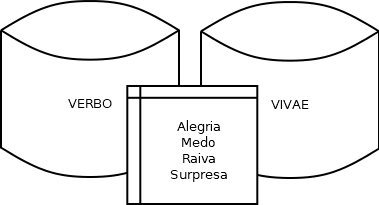
\includegraphics[width=0.40\textwidth]{img/p-yverbointeryvivae.png}
    \caption{\label{fig:yverbointeryvivae}Interseção entre rótulos de emoções de VERBO e VIVAE}
\end{figure}

Vamos redefinir $X_{VERBO} = \{x_i \mid y_i \in Y\}$, analogamente para $X_{VIVAE}$, e vamos definir nosso domínio $X = X_{VERBO} \bigcap X_{VIVAE}$, assim

\begin{itemize}
    \item $\forall x_i \in X, \exists y_i \in Y$ tal que  $y_i$ é a classe de $x_i$
    \item $\forall x_j \in X_{VIVAE}, \exists z_j \in Z$ tal que  $z_j$ é a intensidade de $x_j$
\end{itemize}

Ao realizar tarefas de \textit{DL}, precisamos transformar os dados de entrada em um formato passível de ingestão pelos modelos. Os arquivos \textit{.wav} de $X$ serão lidos e iremos gerar seus respectivos \textit{MFCs}, convertendo o sinal de áudio ao longo do tempo para uma representação do sinal no domínio da frequência, que será utilizada pelos modelos. Então, teremos um mapa $M(x_i): MFC_i$.

\begin{figure}[]
    \centering
    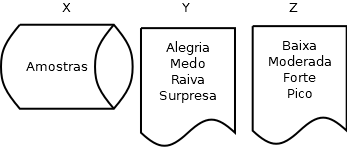
\includegraphics[width=0.5\textwidth]{img/p-dominios-contradominos.png}
    \caption{\label{fig:dominioscontradominios}Domínio e contradomínios}
\end{figure}

% ==========================================================================================
\section{Extração de características}\label{sec:bravo_ae}

De posse do mapa $M(x_i)$, podemos prosseguir para a etapa de extração de características. Apesar da representação visual, os \textit{MFCC}s formam um vetor de alta dimensionalidade. Uma vez que $X$ é formado por dados de \textit{datasets} diferentes, buscamos uma forma de extrair características relevantes com boa capacidade de generalização ao ser aplicada em ambos $X_{VERBO}$ e $X_{VIVAE}$.

Redes neurais constituem uma boa ferramenta para tarefas de \textit{SER}. \textit{Autoencoders}, podem criar uma representação de qualidade com dimensionalidade reduzida em seu espaço latente, enquanto \textit{DNNs} encontram espaço na literatura como bons discriminadores ou classificadores.

Vamos construir um \textit{Autoencoder} ($AE$), exemplificado na Figura \ref{fig:composicaoae}, que tenta reproduzir uma função identidade. Por definição, um \textit{Autoencoder} é composto por uma função \textit{encoder} ($f_e$) e uma função $decoder$ ($f_d$), de modo que $AE: M \rightarrow M'$ faça

\begin{equation}
    AE(x) = f_d(f_e(x)) = x' \approx x
\end{equation}

\begin{figure}[]
    \centering
    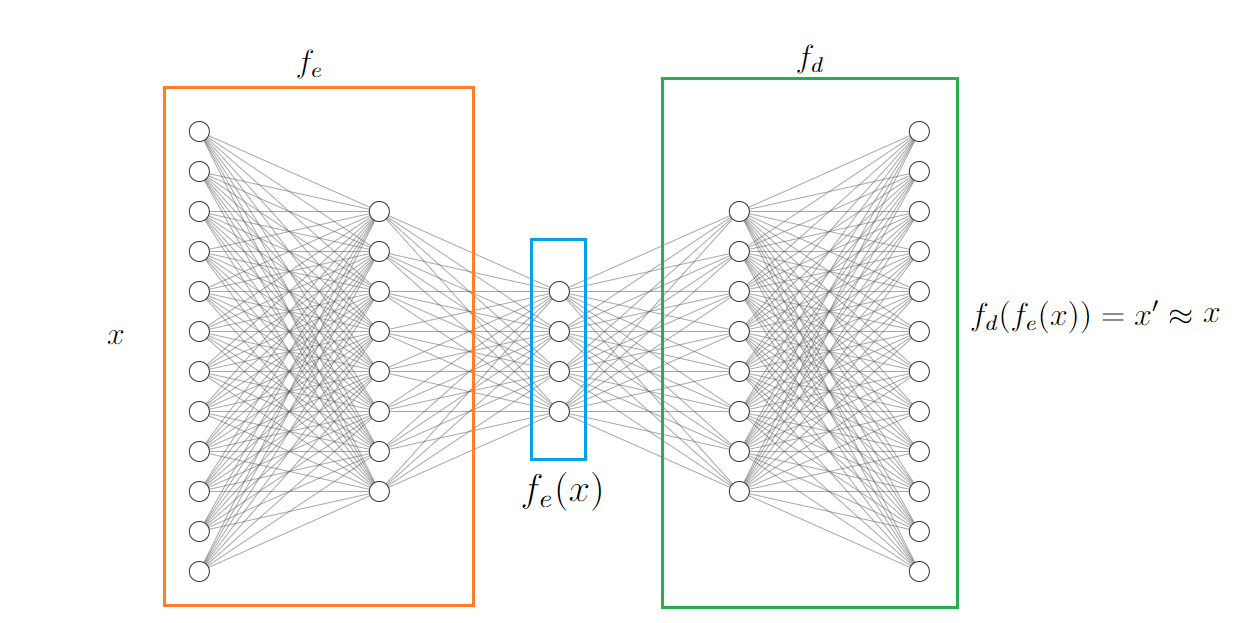
\includegraphics[width=0.9\textwidth]{img/p-autoencoder.png}
    \caption{\label{fig:composicaoae}Composição do \textit{AE}}
\end{figure}

O modelo $AE$ será treinado em $X$, e em seu espaço latente teremos uma representação do dado de entrada com a dimensionalidade reduzida, preservando suas características de maneira suficiente para que possa ser reconstruído ($x'$) ao aplicar a função de \textit{decoding}.

% ==========================================================================================
\section{Classificação da Intensidade}\label{sec:bravo_clf}

Através do modelo de Russel sabemos que que é possível dispor as emoções em função da valência (prazer ou desprazer) e da ativação (vigor ou quietude) ~\cite{27}. Plutchik decompõe as emoções básicas de acordo com a intensidade, chegando a emoções compostas, formadas a partir de duas emoções com intensidades menores.

Ao longo do Capítulo \ref{Cap:Trabalhos Relacionados}, observamos trabalhos relacionados, desafios pertinentes à pesquisa e o estado da arte na área de estudo deste trabalho, que se diferencia dos pares por, além de ser um dos poucos trabalhos a lidar com o idioma português, também aborda a questão da intensidade da emoção.

Sabemos da relevância que \textit{features} espectrais carregam sobre a vocalização e vimos formas para avaliar o desempenho dos modelos. Para a etapa de classificação da intensidade, vamos construir e treinar um modelo supervisionado, uma rede neural conexa $j$, que recebe como \textit{input} o \textit{encoding} da média dos \textit{MFC}s
 dos $x_i \in X_{VIVAE_{treino}}$.

Este modelo (Figura \ref{fig:jsupervisionado}) será construído para classificar a intensidade da emoção de forma direta. Uma vez que os $x_i \in X_{VIVAE_{treino}}$ têm correspondentes em $Z$, contradomínio das intensidades, então, $j: M \rightarrow Z$, é tal que

\begin{equation}
    j(f_e(m)) = z
\end{equation}

\begin{figure}[h]
    \centering
    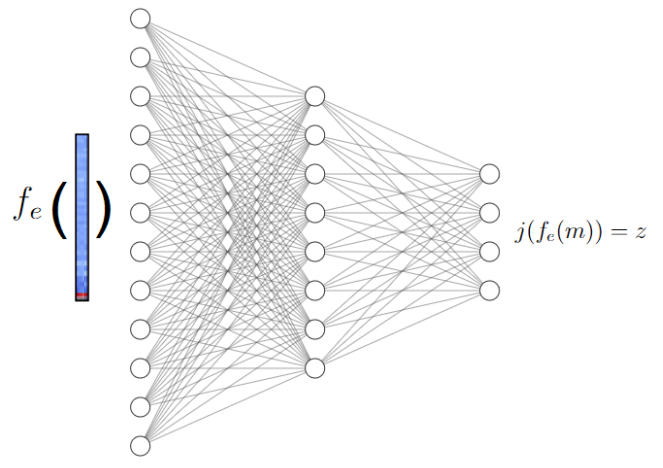
\includegraphics[width=0.75\textwidth]{img/p-supervisionado.png}
    \caption{\label{fig:jsupervisionado}Modelo supervisionado $j$}
\end{figure}

% ==========================================================================================
\section{Validação}\label{sec:bravo_aval}

Modelos de classificação ou regressão precisam ser validados para que possamos avaliar o seu desempenho e gerar inferências a respeito do seu comportamento. Existem diversas formas, algumas expostas em \ref{sec:metricas}, para avaliar seus resultados, sendo esta mais ou menos adequadas à natureza do modelo.

\subsection{Autoencoder}

Antes de seguir para a etapa de classificação (B), precisamos verificar a qualidade do modelo produzido, já que este irá prover os dados para o próximo modelo. Apesar de ser um modelo não supervisionado, podemos pensar em formas de aferir seu desempenho. Uma vez que o modelo \textit{AE} tenta reproduzir a função identidade, podemos calcular a diferença entre os atributos de entrada e os atributos de saída. Para isso, podemos utilizar o Erro Quadrático Médio (\textit{Mean Squared Error, MSE}):

\begin{equation}
    MSE = \frac{1}{n} * \sum^n_{i=1} (x_i - x'_i)^2
\end{equation}

É desejado que o \textit{MSE} para os atributos de $\{x, x'\}$ seja o mais próximo de zero, indicando que o modelo consegue reconstruir o \textit{input} com grande precisão.

Após o treinamento, vamos separar $X_{VIVAE}$ em duas partes, que irão formar as amostras de treino ($X_{VIVAE_{treino}}$) e teste ($X_{VIVAE_{teste}}$), respectivamente, do modelo supervisionado $j$ que iremos construir a seguir.

\subsection{Classificador}

Por ser tratar de um modelo supervisionado, podemos aplicar as métricas descritas em \ref{sec:metricas}, utilizando $X_{VIVAE_{teste}}$ para testar e validar seus resultados. Neste trabalho, perceberemos um erro de  falso negativo com o mesmo peso de um erro de falso positivo. Portanto, não buscamos otimizar as métricas como \textit{Precision} ou \textit{Recall}. Assim, utilizaremos utilizaremos \textit{F1-Score} como parâmetro de desempenho para o modelo supervisionado.
